\documentclass[pdflatex,compress]{beamer}

%\usetheme[dark,framenumber,totalframenumber]{ElektroITK}
\usetheme[darktitle,framenumber,totalframenumber]{ElektroITK}

\usepackage{graphicx}

\title{PEMODELAN JARINGAN KOMUNIKASI}
\subtitle{IP Address Classes}

\author{Mifta Nur Farid, S.T., M.T.}

\begin{document}

\maketitle

\section{Class A IP Addresses}

\begin{frame}
	\frametitle{Subnet Size}
	\begin{center}
		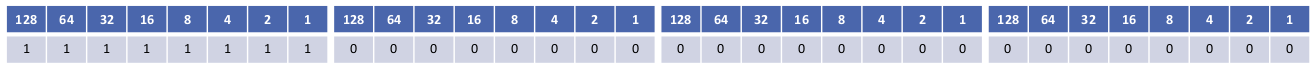
\includegraphics[width=1\linewidth]{img/img01}
	\end{center}
	\begin{itemize}
		\item The bigger the host portion of the network, the more hosts we can have
		\item If the subnet mask is /8, we have 24 bits available to allocate to hosts
		\item If the subnet mask is /24, we only have 8 bits available to allocate to hosts
	\end{itemize}
\end{frame}

\begin{frame}
	\frametitle{How Internet Addressing Was\\Meant to Work}
	\begin{itemize}
		\item The global coordination of Internet IPv4 addressing is performed by IANA (Internet Assigned Numbers Authority).
		\item This is the way it was originally supposed to work:
		\item When a company wants to communicate on the internet, they apply for a range of IP addresses.
		\item If they have 6000 hosts, they ask for a range of IP addresses big enough to cover that, plus room for growth.
		\item They then allocate their addresses to their hosts in their various offices.
	\end{itemize}
\end{frame}

\begin{frame}
	\frametitle{How Internet Addressing Was\\Meant to Work}
	\begin{itemize}
		\item Unfortunately, when IPv4 was created, the designers didn't realise how big the internet was going to get, and they didn't create a big enough address space - there's not enough addresses for everyone.
		\item The long term solution to this problem is IPv6 which has a much bigger address space.
	\end{itemize}
\end{frame}

\begin{frame}
	\frametitle{How Internet Addressing Was\\Meant to Work}
	\begin{itemize}
		\item Private IP addresses with NAT (Network Address Translation) are currently deployed in the majority of enterprise networks as a workaround.
		\item You’ll learn all about private addresses, NAT and IPv6 in a later lecture.
		\item To understand the lectures until we get to that point, think about it from the context of the originally intended IPv4 design, where all hosts which can communicate on the Internet have a public IP address.
	\end{itemize}
\end{frame}

\begin{frame}
	\frametitle{Class A}
	\begin{itemize}
		\item The internet authorities split the IPv4 address space into separate classes.
		\item Class A addresses are assigned to networks with a very large number of hosts.
		\item The high-order (first) bit in a class A address is always set to zero.
		\item The default subnet mask is /8
		\item Valid network addresses range from 1.0.0.0 to 126.0.0.0/8
		\item This allows for 126 networks and 16,777,214 hosts per network.
		\begin{center}
			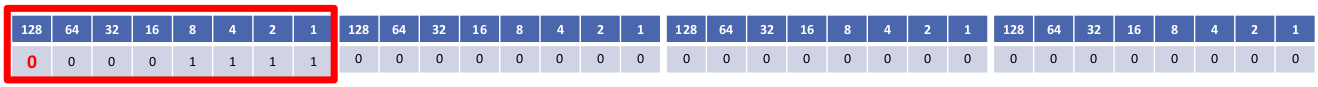
\includegraphics[width=1\linewidth]{img/img02}
		\end{center}
		\item 15.0.0.0/8
	\end{itemize}
\end{frame}

\begin{frame}
	\frametitle{Reserved Class A Addresses}
	\begin{itemize}
		\item 0.0.0.0/8 is reserved and signifies 'this network'
		\item 0.0.0.1 to 0.255.255.255 are not valid host addresses
		\begin{center}
			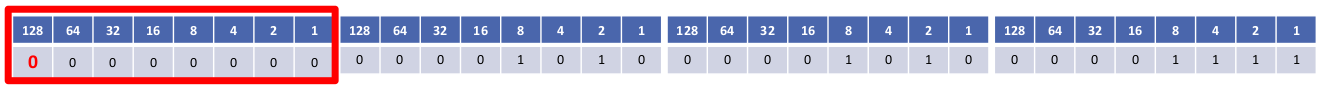
\includegraphics[width=1\linewidth]{img/img03}
		\end{center}
		\item 127.0.0.0/8 in the Class A space is reserved as the loopback address
		for testing the local computer
		\item 127.0.0.1 to 127.255.255.255 are not valid host addresses
		\begin{center}
			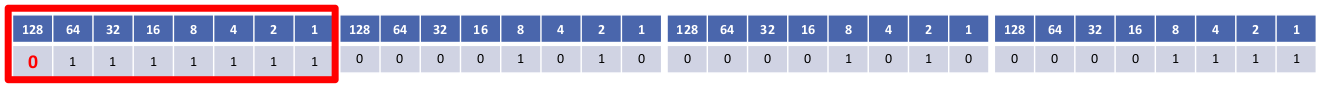
\includegraphics[width=1\linewidth]{img/img04}
		\end{center}
		\item This wiped out 33,554,428 addresses from the global address pool - whoops!
	\end{itemize}
\end{frame}

\begin{frame}
	\frametitle{Subnetting}
	\begin{itemize}
		\item Obviously a company wouldn't put all 16,777,214 hosts into a single logical network, this would be terrible for performance and security.
		\item They would split their /8 address allocation into smaller subnets and allocate these to different offices and types of hosts
		\item For example if they received 15.0.0.0/8, they could allocate the subnet 15.0.1.0/24 to sales computers in New York, 15.0.2.0/24 to accounting PCs and 15.0.9.0/24 to sales computers in Boston.
		\item This is called subnetting and you’ll master it later in this section.
	\end{itemize}
\end{frame}

\end{document}